\documentclass[a4paper, 12pt]{article}
\usepackage[utf8x]{inputenc}
\usepackage[english, russian]{babel}
\usepackage[left=25mm, top=25mm, right=25mm, bottom=25mm]{geometry}
\usepackage{cmap}
\usepackage{indentfirst}
\usepackage{tikz}
\usepackage{float}
\usepackage{amsmath, amsfonts, amssymb}
\usepackage{graphicx}
\usepackage{hyperref}
\usepackage{listings}
\usepackage{caption}
\usepackage{subcaption}
\usepackage{xcolor}
\usepackage{etoolbox}
\usepackage{titlesec}
\pagestyle{plain}
\patchcmd{\tableofcontents}{\contentsname}{\centering\contentsname}{}{}
\titleformat{\section}[block]{\normalfont\large\bfseries\centering}{}{0pt}{}
\titleformat{\subsection}[block]{\normalfont\normalsize\bfseries\centering}{}{0pt}{}
\allowdisplaybreaks
\graphicspath{{src/images/}}
\usetikzlibrary{patterns}
\definecolor{LightGray}{gray}{0.95}
\definecolor{LightGray2}{gray}{0.7}
\lstdefinestyle{code}{
    language=MATLAB, % replace language here
    basicstyle=\footnotesize\ttfamily,
    % numbers=left,
    % numberstyle=\scriptsize\color{gray},
    % stepnumber=1,
    % numbersep=5pt,
    backgroundcolor=\color{LightGray},
    showspaces=false,
    showstringspaces=false,
    showtabs=false,
    tabsize=4,
    captionpos=b,
    breaklines=true,
    breakatwhitespace=false,
    frame=single,
    rulecolor=\color{LightGray2},
    linewidth=\linewidth,
    keywordstyle=\color{blue}\bfseries,
    commentstyle=\color{green!40!black},
    stringstyle=\color{purple},
    escapeinside={\%*}{*)},
    inputencoding=utf8x,
    xleftmargin=0pt,
    framexleftmargin=0pt,
    framexrightmargin=0pt
}
\lstset{style=code}
\hypersetup{
    colorlinks=true,
    linkcolor=blue,
    filecolor=magenta,
    urlcolor=cyan,
    pdftitle={contents setup},
    pdfpagemode=FullScreen,
}


\begin{document}
    \begin{titlepage}

        \begin{center}
        Федеральное государственное автономное образовательное учреждение высшего образования
        «Национальный Исследовательский Университет ИТМО»
        \vfill
        
        
\includegraphics[width=0.3\textwidth]{itmo.png} % requires /src/images/itmo.png

        {\large\bf ЛАБОРАТОРНАЯ РАБОТА №A}\\
        {\large\bf ПРЕДМЕТ «ТЕОРИЯ АВТОМАТИЧЕСКОГО УПРАВЛЕНИЯ»}\\
        {\large\bf ТЕМА «ЛИНЕЙНО-КВАДРАТИЧНЫЕ РАДОСТИ»}\\
        Вариант №2
        \vfill

        \begin{flushright}
            \begin{minipage}{.45\textwidth}
            {
                \hbox{Преподаватель:}
                \hbox{Пашенко А. В.}
                \hbox{}
                \hbox{Выполнил:}
                \hbox{Румянцев А. А.}
                \hbox{}
                \hbox{Факультет: СУиР}
                \hbox{Группа: R3341}
                \hbox{Поток: ТАУ R22 бак 1.1.1}
            }
            \end{minipage}
        \end{flushright}
        \vfill
  
        Санкт-Петербург\\
        2025
        \end{center}
    \end{titlepage}
    
    \tableofcontents

    \newpage
    \section{Задание 1. Исследование LQR}
    Рассмотрим систему
    $$
    \dot{x}=Ax+Bu,\ x(0)=\begin{bmatrix}
        1\\1\\1
    \end{bmatrix},\ A=\begin{bmatrix}
        5 &2 &7\\
        2 &1 &2\\
        -2 &-3 &-4
    \end{bmatrix},\ B=\begin{bmatrix}
        3\\1\\-1
    \end{bmatrix};
    $$


    \subsection{Стабилизируемость системы}
    Проверим систему на стабилизируемость. Найдем собственные
    числа матрицы $A$. Ранее мы это делали в лабораторной работе
    №2 <<Модальные регуляторы и наблюдатели>>.
    Код матлаб представлен в приложении А на листинге \ref{task1}
    $$
    \sigma\left( A \right)=\left\{ -2,2\pm i \right\}
    $$
    Собственное число $\lambda_1=-2$ асимптотически устойчивое,
    может быть неуправляемым. Комплексная пара $\lambda_{2,3}=2\pm i$
    неустойчива, нужна управляемость. Разложим $A$ в ЖНФ в вещественном
    виде, найдем $B$ в базисе собственных векторов $A$
    $$
    A_{J_{re}}=\begin{bmatrix}
    -2     &0     &0\\
    0     &2     &1\\
    0    &-1     &2
    \end{bmatrix},\ B_{J_{re}}=\begin{bmatrix}
        0\\3\\-1
    \end{bmatrix};
    $$
    Система не полностью управляема, стабилизируема (собственному
    значению $-2$ соответствует ноль в матрице $B_{J_{re}}$).
    

    \subsection{Схема моделирования системы}
    Построим схему моделирования системы, замкнутой регулятором $u=Kx$,
    используя \texttt{SIMULINK}
    \begin{figure}[H]
        \centering
        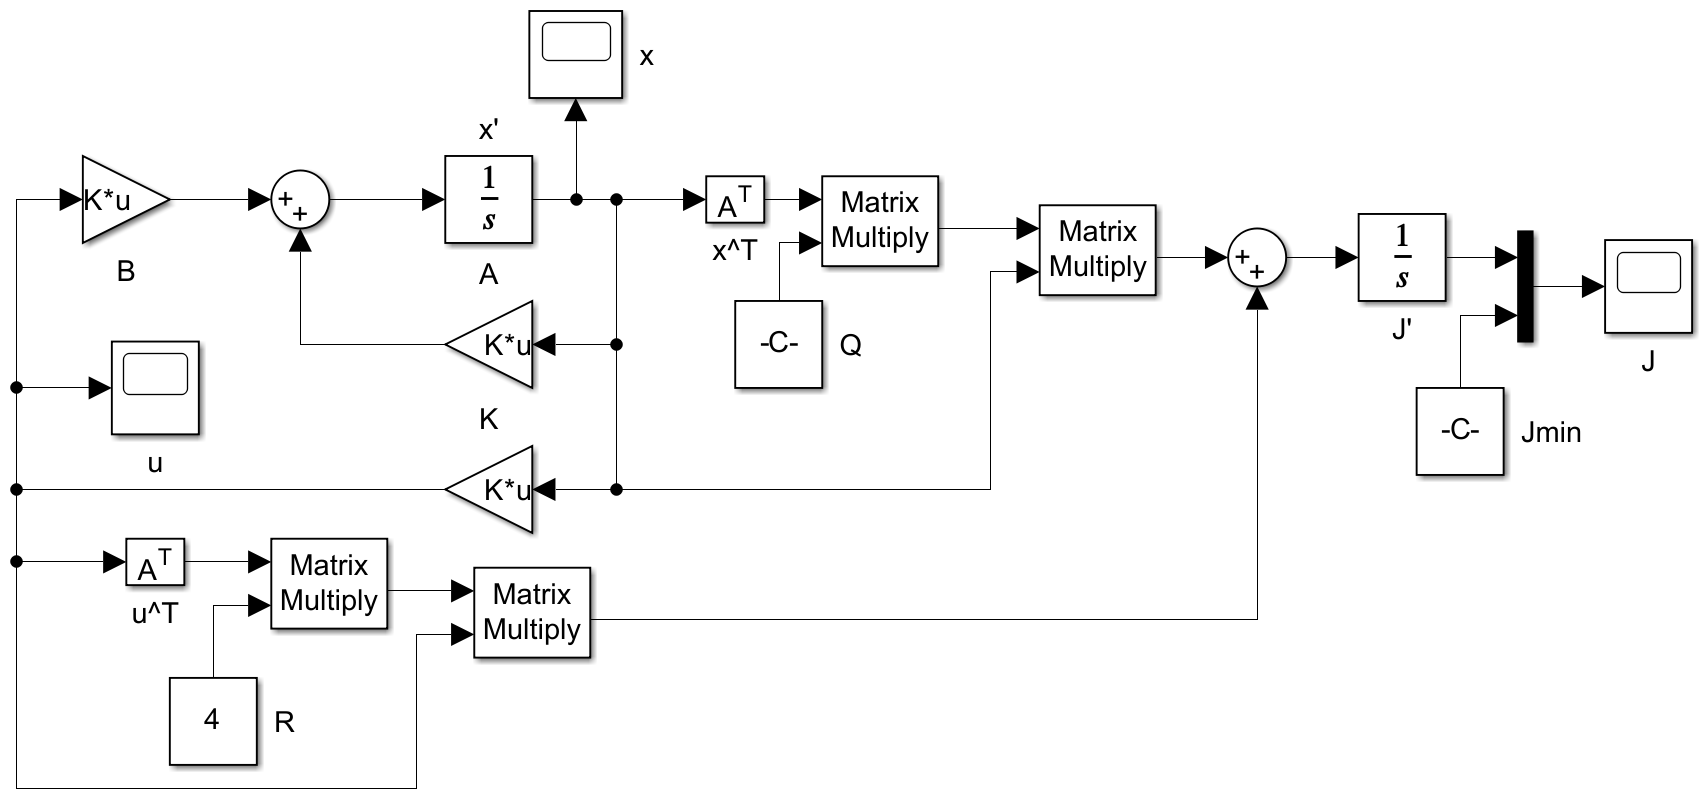
\includegraphics[scale=0.35]{1task_scheme.png}
        \captionsetup{skip=0pt}
        \caption{Схема моделирования системы, замкнутой регулятором}
        \label{fig:1task_scheme}
    \end{figure}
    Снимаем осциллограммы $u(t),x(t),J_{exp}(t)$.


    \subsection{Набор пар матриц для исследования}
    Зададим значения матриц $Q=I,R=1$ (время процесса и затраты на управление принимаем одинаково значимыми) и параметр $\alpha=4$.
    Таким образом, сформируем набор
    \begin{align*}
        &\circ \left( Q=I, R=1 \right),\\
        &\circ \left( Q=4I, R=1 \right),\\
        &\circ \left( Q=I, R=4 \right),\\
        &\circ \left( Q=4I, R=4 \right);
    \end{align*}


    \subsection{Синтез регулятора}
    Для каждой из пар значений матриц $\left( Q,R \right)$ синтезируем
    регулятор, минимизирующий функционал качества
    $$
    J=\int\limits_{0}^{\infty}\left( x^T(t)Qx(t)+u^T(t)Ru(t) \right)dt
    $$
    путем решения соответствующего матричного уравнения Риккати при $\nu=1$
    $$
    A^TP+PA+Q-\nu PBR^{-1}B^TP=0,\ K=-R^{-1}B^TP;
    $$
    Воспользуемся \texttt{icare} и получим
    \begin{align*}
        &\left( Q=I, R=1 \right),\ K_{I,1}=\begin{bmatrix}
            -1.7473 &-5.4627 &-1.4004
        \end{bmatrix},\\
        &\left( Q=4I, R=1 \right),\ K_{4I,1}=\begin{bmatrix}
            -2.0000 &-6.9630 &-0.9630
        \end{bmatrix},\\
        &\left( Q=I, R=4 \right),\ K_{I,4}=\begin{bmatrix}
            -1.6433 &-4.9797 &-1.5454
        \end{bmatrix},\\
        &\left( Q=4I, R=4 \right),\ K_{4I,4}=\begin{bmatrix}
            -1.7473 &-5.4627 &-1.4004
        \end{bmatrix};
    \end{align*}
    Убедимся, что спектры замкнутых систем принадлежат левой комплексной полуплоскости
    \begin{align*}
        &\sigma\left( A+BK_{I,1} \right)=\left\{ -2,-1.4413,-3.8630 \right\},\\
        &\sigma\left( A+BK_{4I,1} \right)=\left\{ -2,-1,-7 \right\},\\
        &\sigma\left( A+BK_{I,4} \right)=\left\{ -2,-2.1821\pm0.6216i \right\},\\
        &\sigma\left( A+BK_{4I,4} \right)=\left\{ -2,-1.4413,-3.8630 \right\};
    \end{align*}
    Получили отрицательные действительные части собственных чисел и наличие в спектрах неуправляемого $\lambda_1=-2$.
    Следовательно, регуляторы синтезированы корректно.


    \subsection{Минимизированное значение функционала качества}
    Вычислим минимизированное значение функционала качества
    $$
    J_{min}=x_0^TPx_0
    $$
    для каждой пары $\left( Q,R \right)$. $P_i$ получили при решении
    матричного уравнения типа Риккати
    $$
    P_{I,1}=\begin{bmatrix}
        2.4681   &-3.5514    &2.1055\\
        -3.5514   &13.4136   &-2.7033\\
         2.1055   &-2.7033    &2.2129   
    \end{bmatrix},\ P_{4I,1}=\begin{bmatrix}
        4.0000   &-7.3333   & 2.6667\\
   -7.3333   &24.9904   &-3.9726\\
    2.6667   &-3.9726    &3.0645
    \end{bmatrix},
    $$
    $$
    P_{I,4}=\begin{bmatrix}
        8.2455  &-10.2978    &7.8656\\
  -10.2978   &41.3731   &-9.4392\\
    7.8656   &-9.4392    &7.9761   
    \end{bmatrix},\ P_{4I,4}=\begin{bmatrix}
        9.8723  &-14.2056    &8.4221\\
  -14.2056   &53.6545  &-10.8133\\
    8.4221  &-10.8133    &8.8515
    \end{bmatrix};
    $$
    Получаем
    \begin{align*}
        &Q=I,R=1:\ J_{min}=9.7962,\\
        &Q=4I,R=1:\ J_{min}=14.7764,\\
        &Q=I,R=4:\ J_{min}=33.8518,\\
        &Q=4I,R=4:\ J_{min}=39.1846;
    \end{align*}


    \subsection{Компьютерное моделирование}
    Выполним компьютерное моделирование замкнутых систем и для каждого случая построим
    график управления $u(t)$, вектора состояния замкнутой системы $x(t)$
    и экспериментального значения функционала качества $J_{exp}(t)$. Моделирование
    $u(t)$ и $x(t)$ для случая $$Q=4I,R=4,K_{4I,4}=\begin{bmatrix}
        -1.7473 &-5.4627 &-1.4004
    \end{bmatrix}$$ делать не будем, так как регулятор для
    этой пары совпал с регулятором для случая $$Q=I,R=1,K_{I,1}=\begin{bmatrix}
        -1.7473 &-5.4627 &-1.4004
    \end{bmatrix},$$ собственные числа тоже одинаковые. Результаты представлены на
    рис. \ref{fig:1task_u}--\ref{fig:1task_jjjj}
    \begin{figure}[H]
        \centering
        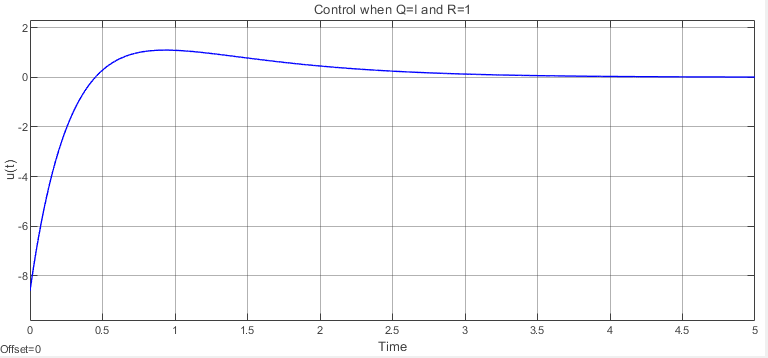
\includegraphics[scale=0.75]{1task_u.png}
        \captionsetup{skip=0pt}
        \caption{График управления $u(t)$ при $K_{I,1},K_{4I,4}$}
        \label{fig:1task_u}
    \end{figure}
    \begin{figure}[H]
        \centering
        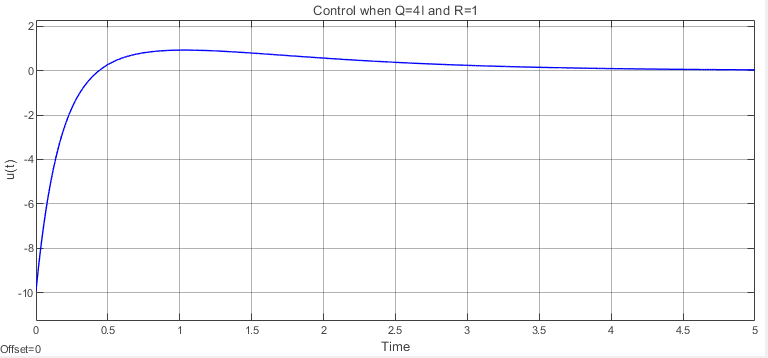
\includegraphics[scale=0.75]{1task_uu.png}
        \captionsetup{skip=0pt}
        \caption{График управления $u(t)$ при $K_{4I,1}$}
        \label{fig:1task_uu}
    \end{figure}
    \begin{figure}[H]
        \centering
        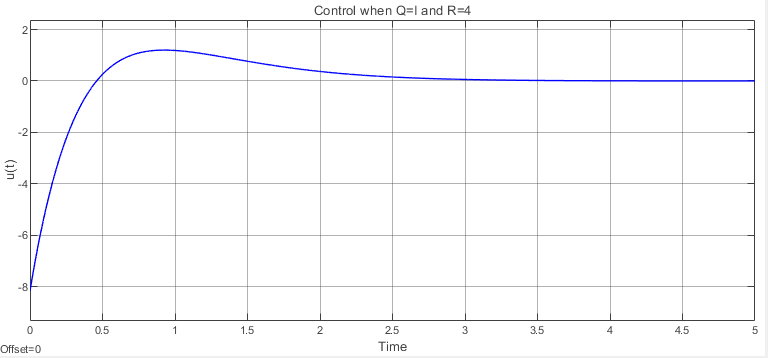
\includegraphics[scale=0.75]{1task_uuu.png}
        \captionsetup{skip=0pt}
        \caption{График управления $u(t)$ при $K_{I,4}$}
        \label{fig:1task_uuu}
    \end{figure}
    \begin{figure}[H]
        \centering
        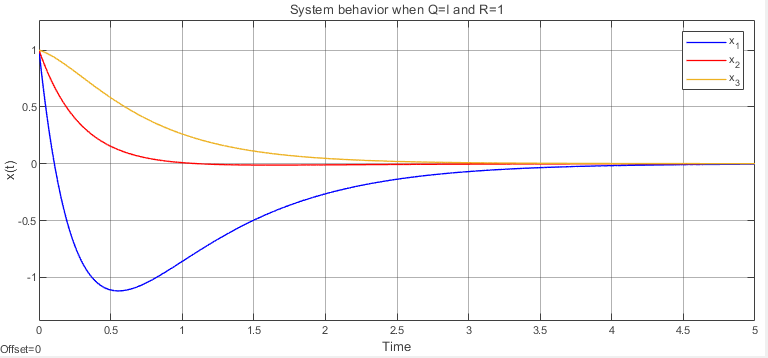
\includegraphics[scale=0.75]{1task_x.png}
        \captionsetup{skip=0pt}
        \caption{График вектора состояния $x(t)$ при $K_{I,1},K_{4I,4}$}
        \label{fig:1task_x}
    \end{figure}
    \begin{figure}[H]
        \centering
        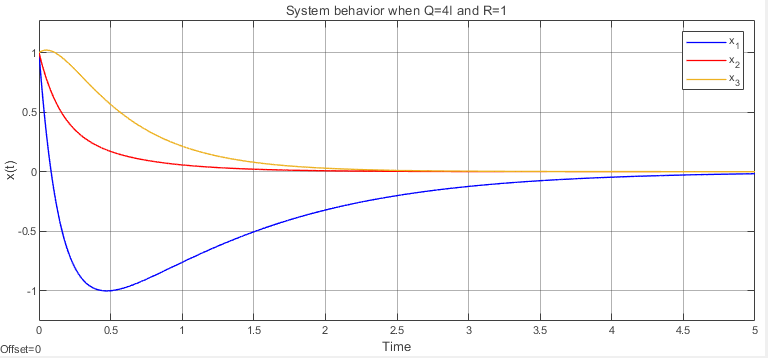
\includegraphics[scale=0.75]{1task_xx.png}
        \captionsetup{skip=0pt}
        \caption{График вектора состояния $x(t)$ при $K_{4I,1}$}
        \label{fig:1task_xx}
    \end{figure}
    \begin{figure}[H]
        \centering
        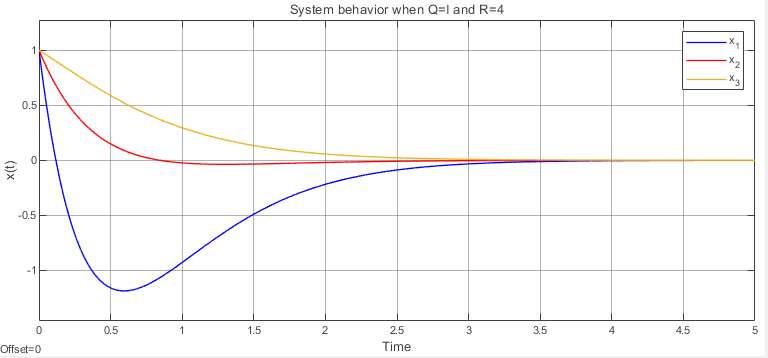
\includegraphics[scale=0.75]{1task_xxx.png}
        \captionsetup{skip=0pt}
        \caption{График вектора состояния $x(t)$ при $K_{I,4}$}
        \label{fig:1task_xxx}
    \end{figure}
    \begin{figure}[H]
        \centering
        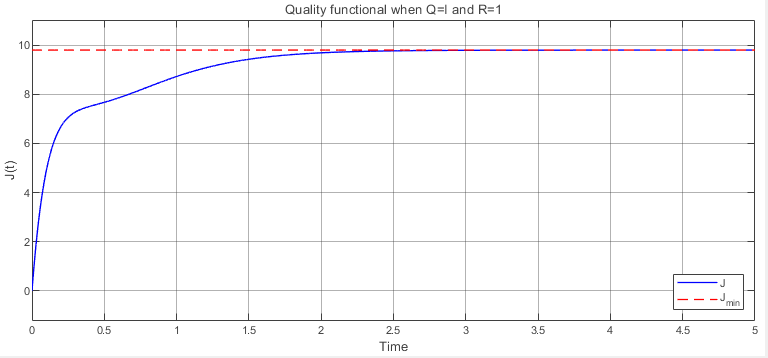
\includegraphics[scale=0.75]{1task_j.png}
        \captionsetup{skip=0pt}
        \caption{График экспериментального значения функционала качества $J(t)$ при $K_{I,1}$}
        \label{fig:1task_j}
    \end{figure}
    \begin{figure}[H]
        \centering
        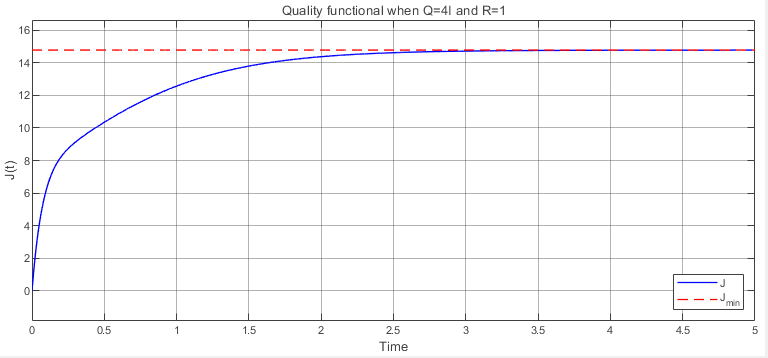
\includegraphics[scale=0.75]{1task_jj.png}
        \captionsetup{skip=0pt}
        \caption{График экспериментального значения функционала качества $J(t)$ при $K_{4I,1}$}
        \label{fig:1task_jj}
    \end{figure}
    \begin{figure}[H]
        \centering
        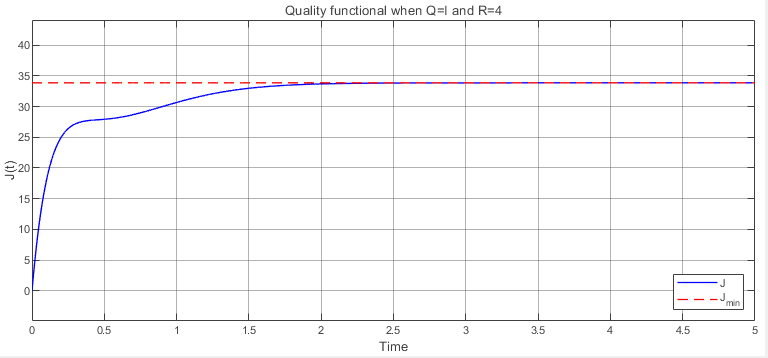
\includegraphics[scale=0.75]{1task_jjj.png}
        \captionsetup{skip=0pt}
        \caption{График экспериментального значения функционала качества $J(t)$ при $K_{I,4}$}
        \label{fig:1task_jjj}
    \end{figure}
    \begin{figure}[H]
        \centering
        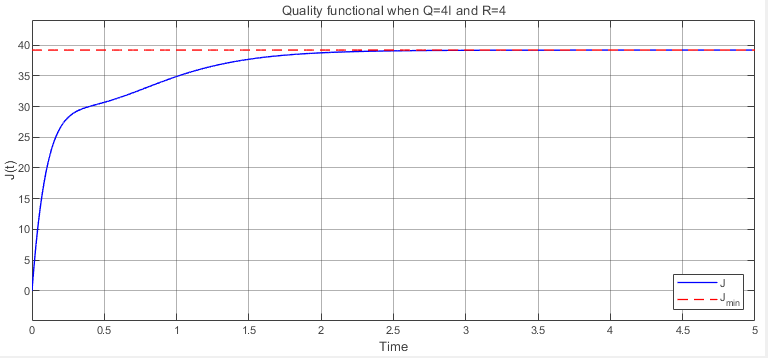
\includegraphics[scale=0.75]{1task_jjjj.png}
        \captionsetup{skip=0pt}
        \caption{График экспериментального значения функционала качества $J(t)$ при $K_{4I,4}$}
        \label{fig:1task_jjjj}
    \end{figure}


    \subsection{Сравнение результатов}
    Когда нам важнее время процесса, чем затраты на управление $(Q>R)$, то
    ожидаемо управления применяется больше (сравн. рис. \ref{fig:1task_uu}, \ref{fig:1task_uuu}),
    при этом координаты $x_2(t),x_3(t)$ вектора состояния объекта быстрее сходятся к нулю (сравн. рис. \ref{fig:1task_xx}, \ref{fig:1task_xxx};
    примечание: координата $x_1(t)$ сравнительно быстрее бы сошлась к нулю при б\'{о}льшем коэффициенте $\alpha$).
    При $Q<R$ ситуация обратная -- время процесса не так важно, как затраты на управление (сравн. те же графики).
    При равнозначных (равносильных) значениях $Q,R$ результат усредненный между временем процесса и затратами на управление.
    Результаты $J_{exp}(t)$ примерно совпадают с вычисленными $J_{min}$. При этом
    $$J_{min,I,1}=\dfrac{J_{min,4I,4}}{4},\ 9.7962\approx\dfrac{39.1846}{4}=9.79615,$$ то есть при увеличении
    $Q,R$ в один и тот же коэффициент $\alpha$, минимизированное значение функционала качества увеличится в
    $\alpha$ раз.


    \section{Задание 2. Исследование фильтра Калмана}
    Рассмотрим систему
    $$
    \begin{cases}
        \dot{x}=Ax+f,\\
        y=Cx+\xi,
    \end{cases} x(0)=\begin{bmatrix}
        1\\1\\1\\1
    \end{bmatrix},\ A=\begin{bmatrix}
        0 &1 &0 &1\\
        -26 &-7 &20 &-11\\
        0 &1 &-1 &2\\
        16 &4 &-14 &8
    \end{bmatrix},\ C=\begin{bmatrix}
        -1 &0 &1 &-1
    \end{bmatrix},
    $$
    где $f(t)$ и $\xi(t)$ -- \textit{случайные} сигналы (гауссовский белый шум) -- исследуем \textit{фильтр Калмана}.


    \subsection{Обнаруживаемость системы}
    Проверим собственные числа матрицы $A$. Программа \texttt{MATLAB} представлена
    в приложении Б на листинге \ref{task2}
    $$
    \sigma\left( A \right)=\left\{ \pm i,\pm2i \right\}
    $$
    Собственные числа устойчивые, но не асимптотически. Проверим наблюдаемость через
    вещественную ЖНФ
    $$
    A_{J_{re}}=\begin{bmatrix}
        0    &2   &0    &0\\
   -2   &0    &0   &0\\
    0   &0    &0    &1\\
   0   &0   &-1   &0
    \end{bmatrix},\ C_{J_{re}}=\begin{bmatrix}
        -0.5   &-0.5   &-0.5  &0
    \end{bmatrix};
    $$
    Комплексные пары наблюдаемы -- система полностью наблюдаема и стабилизируема.


    \subsection{Схема моделирования системы}
    Построим схему моделирования системы с наблюдателем состояния
    $$\dot{\hat{x}}=A\hat{x}+L\left( C\hat{x}-y \right)$$
    Снимаем осциллограммы $x(t),\hat{x}(t),e(t)$
    \begin{figure}[H]
        \centering
        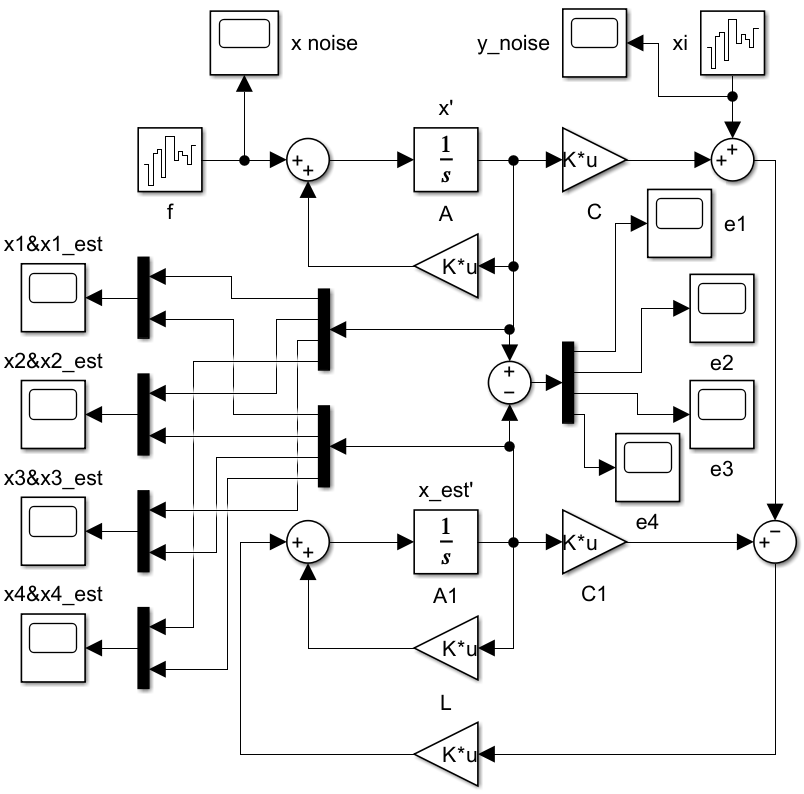
\includegraphics[scale=0.45]{2task_scheme.png}
        \captionsetup{skip=0pt}
        \caption{Схема моделирования системы с наблюдателем состояния}
        \label{fig:2task_scheme}
    \end{figure}


    \subsection{Набор пар матриц для исследования}
    Зададим значения матриц $Q=I,R=1$ (считаем помехи для $x(t)$ и $y(t)$ равнозначными)
    и параметр $\alpha=100$. Таким образом, сформируем набор
    \begin{align*}
        &\circ \left( Q=I, R=1 \right),\\
        &\circ \left( Q=100I, R=1 \right),\\
        &\circ \left( Q=I, R=100 \right),\\
        &\circ \left( Q=100I, R=100 \right);
    \end{align*}


    \subsection{Синтез наблюдателя}
    Для каждой из пар значений матриц $\left( Q,R \right)$ синтезируем
    наблюдатель, минимизирующий средний квадрат отклонения установившейся ошибки наблюдателя
    $$
    \lim\limits_{t\to\infty}\mathbb{E}\left( ||x(t)-\hat{x}(t)||^2 \right)
    $$
    путем решения соответствующего матричного уравнения Риккати при $\nu=1$
    $$
    AP+PA^T+Q-\nu PC^TR^{-1}CP=0,\ L=-PC^TR^{-1};
    $$
    Воспользуемся \texttt{icare} и получим
    \begin{align*}
        &\left( Q=I, R=1 \right),\ L_{I,1}=\begin{bmatrix}
            0.5233  &-7.6440 &0.0221 &6.4594
        \end{bmatrix}^T,\\
        &\left( Q=100I, R=1 \right),\ L_{100I,1}=\begin{bmatrix}
            7.6954 &-15.6987 &-4.5805 &15.1421
        \end{bmatrix}^T,\\
        &\left( Q=I, R=100 \right),\ L_{I,100}=\begin{bmatrix}
            0.0079 &-1.7287 &0.5099 &2.0960
        \end{bmatrix}^T,\\
        &\left( Q=100I, R=4 \right),\ L_{100I,100}=\begin{bmatrix}
            0.5233  &-7.6440 &0.0221 &6.4594
        \end{bmatrix}^T;
    \end{align*}
    Убедимся, что спектры замкнутых систем принадлежат левой комплексной полуплоскости
    \begin{align*}
        &\sigma\left( A+L_{I,1}C \right)=\left\{ -0.3454\pm1.4689i, -3.1349\pm3.3599i \right\},\\
        &\sigma\left( A+L_{100I,1}C \right)=\left\{ -0.3419\pm1.4702i, -13.3670\pm5.6243i \right\},\\
        &\sigma\left( A+L_{I,100}C \right)=\left\{ -0.4006\pm1.1676i,-0.3965\pm1.9848i \right\},\\
        &\sigma\left( A+L_{100I,100}C \right)=\left\{ -0.3454\pm1.4689i, -3.1349\pm3.3599i \right\};
    \end{align*}
    Получили отрицательные действительные части собственных чисел.
    Следовательно, наблюдатели синтезированы корректно.


    \subsection{Компьютерное моделирование}
    Выполним компьютерное моделирование с нулевыми начальными условиями наблюдателя.
    Построим графики $x(t)$, $\hat{x}(t)$, $e(t)$.
    Также приведены графики шумов $f(t)$, $\xi(t)$. Наблюдатели $L_{I,1},L_{100I,100}$ совпали аналогично регуляторам в задании 1
    \begin{figure}[H]
        \centering
        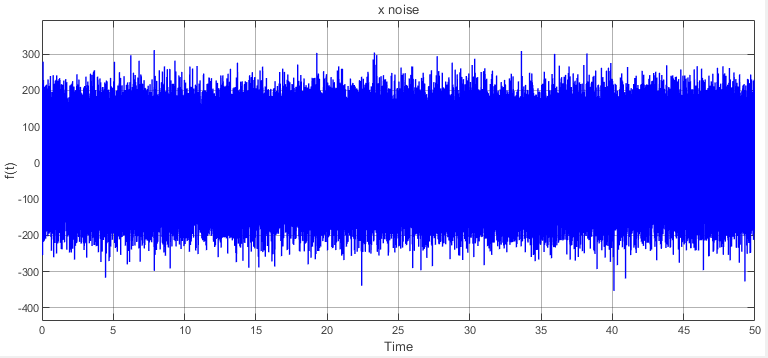
\includegraphics[scale=0.75]{2task_x_noise.png}
        \captionsetup{skip=0pt}
        \caption{График шума $f(t)$}
        \label{fig:2task_x_noise}
    \end{figure}
    \begin{figure}[H]
        \centering
        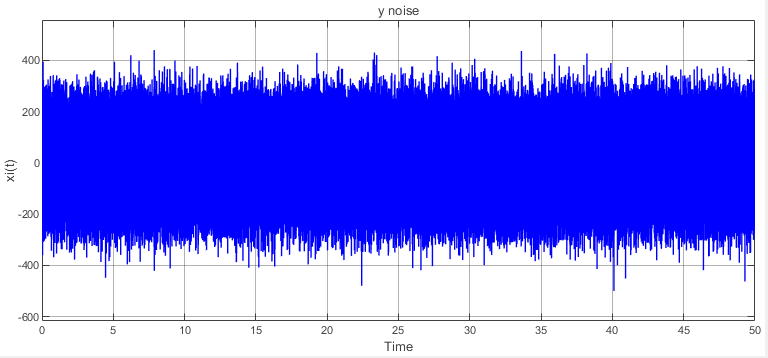
\includegraphics[scale=0.75]{2task_y_noise.png}
        \captionsetup{skip=0pt}
        \caption{График шума $\xi(t)$}
        \label{fig:2task_y_noise}
    \end{figure}
    \begin{figure}[H]
        \centering
        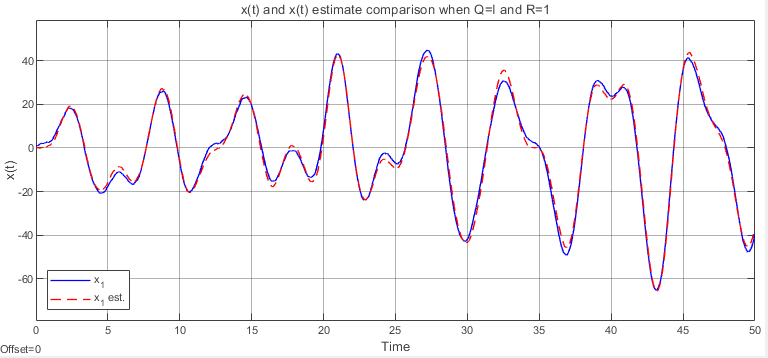
\includegraphics[scale=0.75]{2task_x1.png}
        \captionsetup{skip=0pt}
        \caption{График $x_1(t),\hat{x}_1(t)$ при $L_{I,1},L_{100I,100}$}
        \label{fig:2task_x1}
    \end{figure}
    \begin{figure}[H]
        \centering
        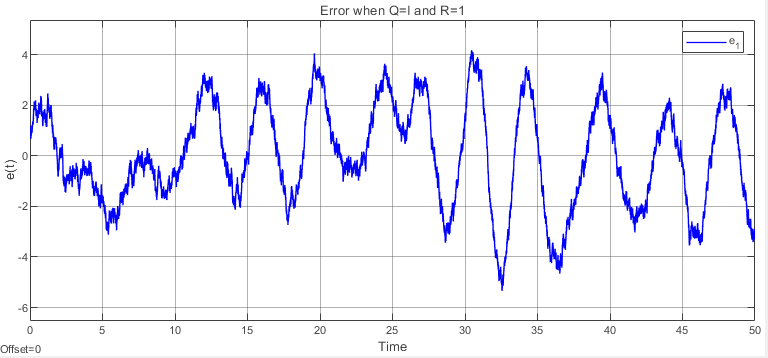
\includegraphics[scale=0.75]{2task_e1.png}
        \captionsetup{skip=0pt}
        \caption{График $e_1(t)=x_1(t)-\hat{x}_1(t)$ при $L_{I,1},L_{100I,100}$}
        \label{fig:2task_e1}
    \end{figure}
    \begin{figure}[H]
        \centering
        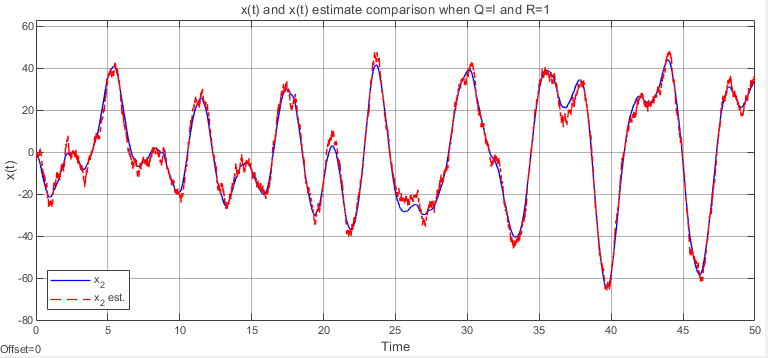
\includegraphics[scale=0.75]{2task_x2.png}
        \captionsetup{skip=0pt}
        \caption{График $x_2(t),\hat{x}_2(t)$ при $L_{I,1},L_{100I,100}$}
        \label{fig:2task_x2}
    \end{figure}
    \begin{figure}[H]
        \centering
        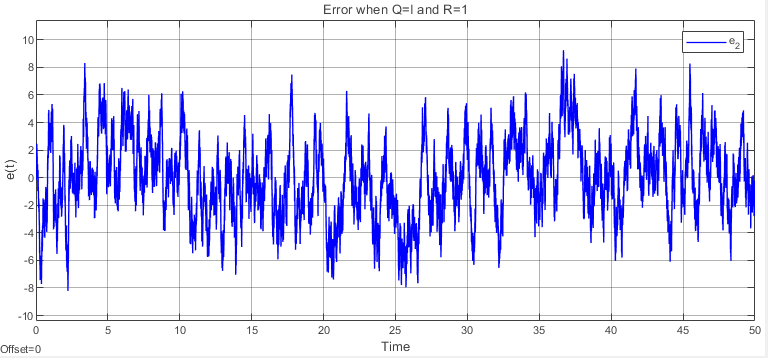
\includegraphics[scale=0.75]{2task_e2.png}
        \captionsetup{skip=0pt}
        \caption{График $e_2(t)=x_2(t)-\hat{x}_2(t)$ при $L_{I,1},L_{100I,100}$}
        \label{fig:2task_e2}
    \end{figure}
    \begin{figure}[H]
        \centering
        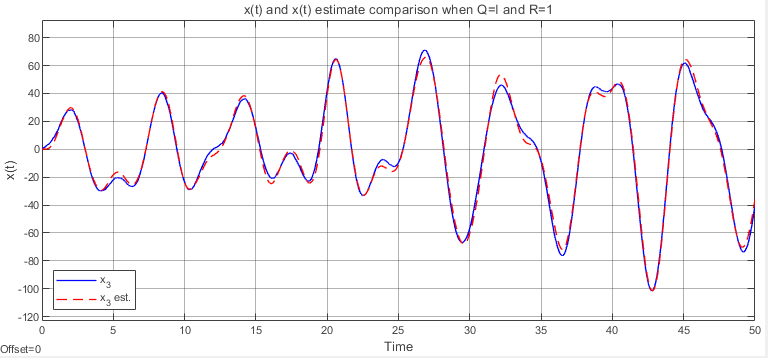
\includegraphics[scale=0.75]{2task_x3.png}
        \captionsetup{skip=0pt}
        \caption{График $x_3(t),\hat{x}_3(t)$ при $L_{I,1},L_{100I,100}$}
        \label{fig:2task_x3}
    \end{figure}
    \begin{figure}[H]
        \centering
        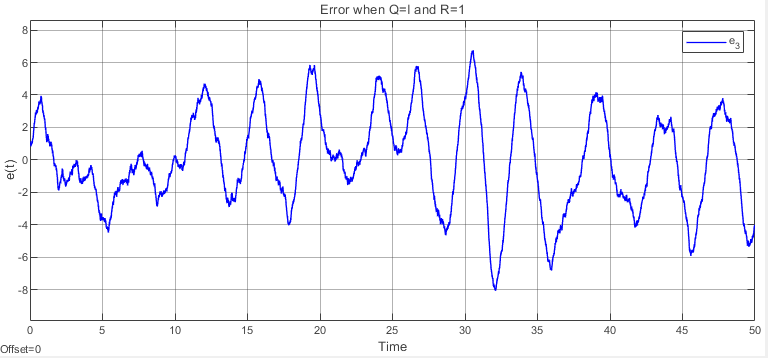
\includegraphics[scale=0.75]{2task_e3.png}
        \captionsetup{skip=0pt}
        \caption{График $e_3(t)=x_3(t)-\hat{x}_3(t)$ при $L_{I,1},L_{100I,100}$}
        \label{fig:2task_e3}
    \end{figure}
    \begin{figure}[H]
        \centering
        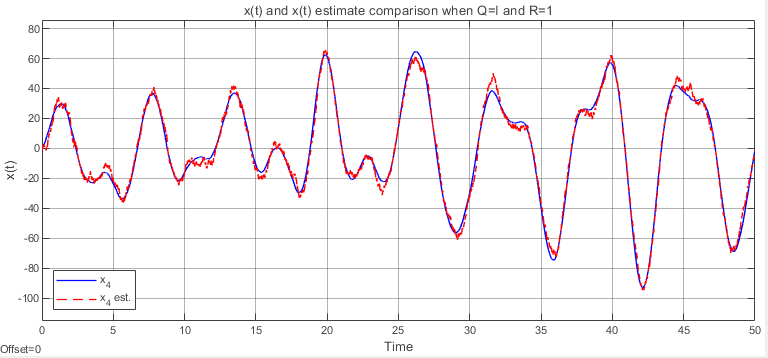
\includegraphics[scale=0.75]{2task_x4.png}
        \captionsetup{skip=0pt}
        \caption{График $x_4(t),\hat{x}_4(t)$ при $L_{I,1},L_{100I,100}$}
        \label{fig:2task_x4}
    \end{figure}
    \begin{figure}[H]
        \centering
        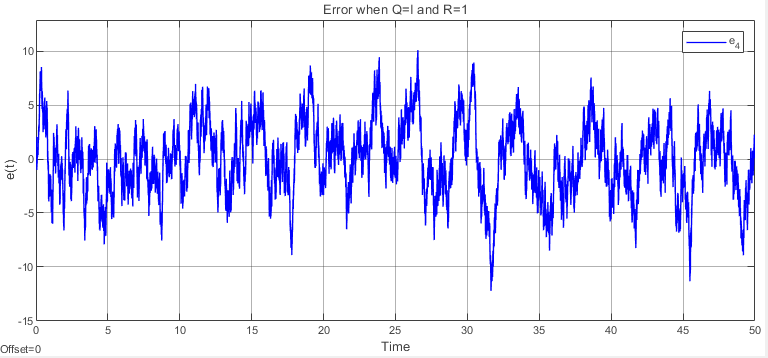
\includegraphics[scale=0.75]{2task_e4.png}
        \captionsetup{skip=0pt}
        \caption{График $e_4(t)=x_4(t)-\hat{x}_4(t)$ при $L_{I,1},L_{100I,100}$}
        \label{fig:2task_e4}
    \end{figure}
    \begin{figure}[H]
        \centering
        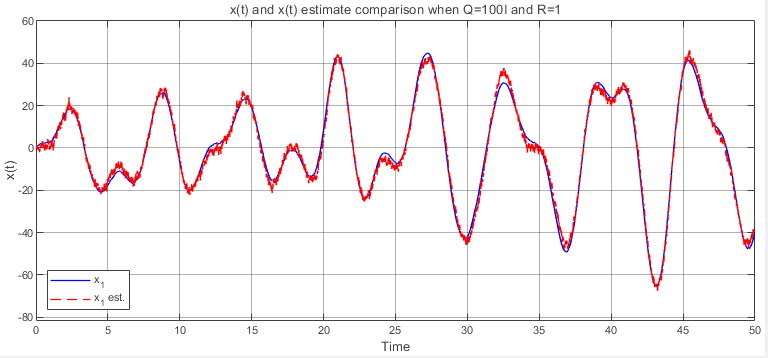
\includegraphics[scale=0.75]{2task_xx1.png}
        \captionsetup{skip=0pt}
        \caption{График $x_1(t),\hat{x}_1(t)$ при $L_{100I,1}$}
        \label{fig:2task_xx1}
    \end{figure}
    \begin{figure}[H]
        \centering
        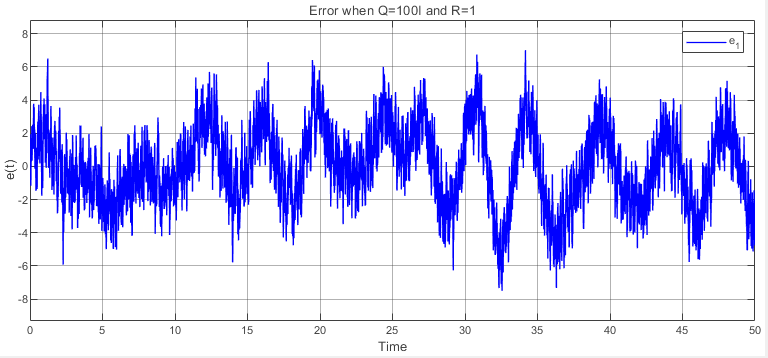
\includegraphics[scale=0.75]{2task_ee1.png}
        \captionsetup{skip=0pt}
        \caption{График $e_1(t)=x_1(t)-\hat{x}_1(t)$ при $L_{100I,1}$}
        \label{fig:2task_ee1}
    \end{figure}
    \begin{figure}[H]
        \centering
        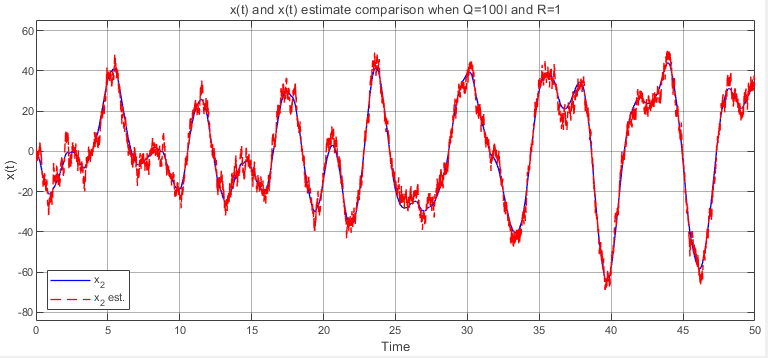
\includegraphics[scale=0.75]{2task_xx2.png}
        \captionsetup{skip=0pt}
        \caption{График $x_2(t),\hat{x}_2(t)$ при $L_{100I,1}$}
        \label{fig:2task_xx2}
    \end{figure}
    \begin{figure}[H]
        \centering
        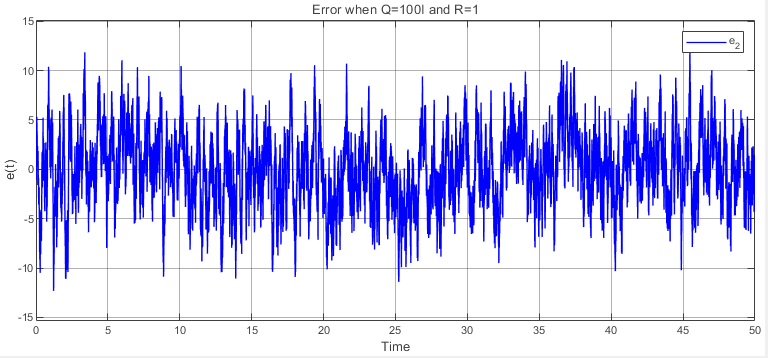
\includegraphics[scale=0.75]{2task_ee2.png}
        \captionsetup{skip=0pt}
        \caption{График $e_2(t)=x_2(t)-\hat{x}_2(t)$ при $L_{100I,1}$}
        \label{fig:2task_ee2}
    \end{figure}
    \begin{figure}[H]
        \centering
        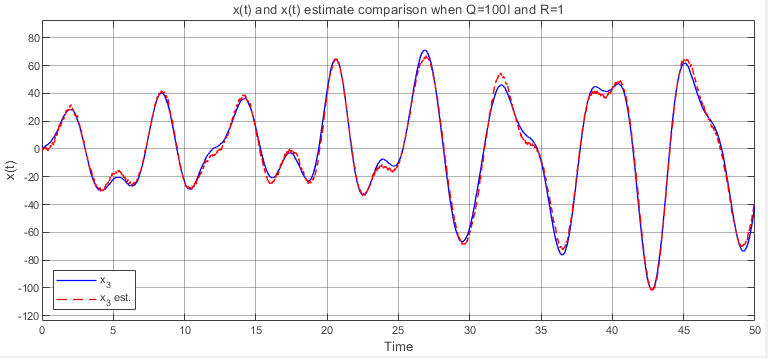
\includegraphics[scale=0.75]{2task_xx3.png}
        \captionsetup{skip=0pt}
        \caption{График $x_3(t),\hat{x}_3(t)$ при $L_{100I,1}$}
        \label{fig:2task_xx3}
    \end{figure}
    \begin{figure}[H]
        \centering
        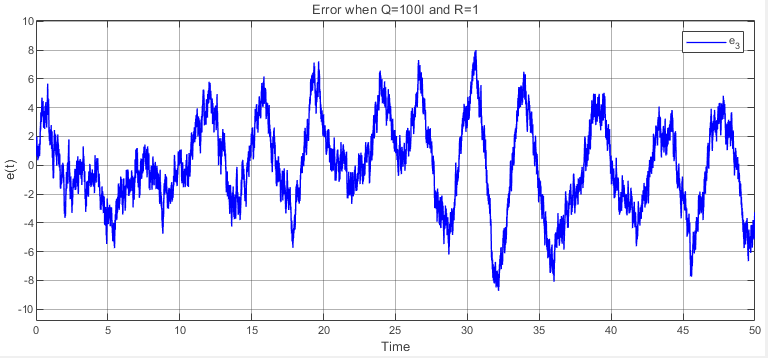
\includegraphics[scale=0.75]{2task_ee3.png}
        \captionsetup{skip=0pt}
        \caption{График $e_3(t)=x_3(t)-\hat{x}_3(t)$ при $L_{100I,1}$}
        \label{fig:2task_ee3}
    \end{figure}
    \begin{figure}[H]
        \centering
        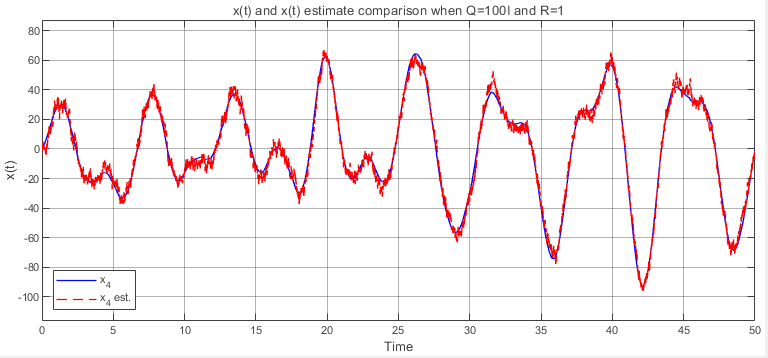
\includegraphics[scale=0.75]{2task_xx4.png}
        \captionsetup{skip=0pt}
        \caption{График $x_4(t),\hat{x}_4(t)$ при $L_{100I,1}$}
        \label{fig:2task_xx4}
    \end{figure}
    \begin{figure}[H]
        \centering
        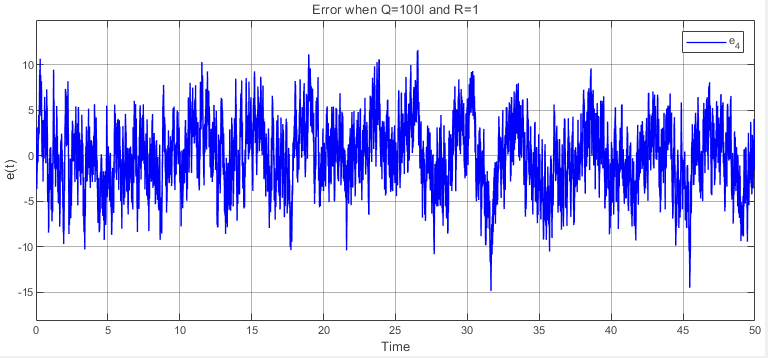
\includegraphics[scale=0.75]{2task_ee4.png}
        \captionsetup{skip=0pt}
        \caption{График $e_4(t)=x_4(t)-\hat{x}_4(t)$ при $L_{100I,1}$}
        \label{fig:2task_ee4}
    \end{figure}
    \begin{figure}[H]
        \centering
        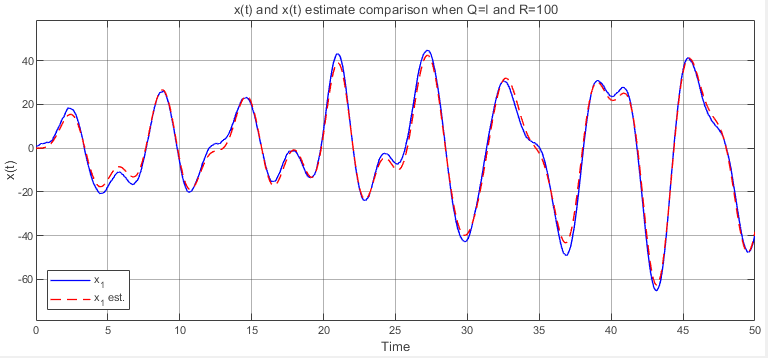
\includegraphics[scale=0.75]{2task_xxx1.png}
        \captionsetup{skip=0pt}
        \caption{График $x_1(t),\hat{x}_1(t)$ при $L_{I,100}$}
        \label{fig:2task_xxx1}
    \end{figure}
    \begin{figure}[H]
        \centering
        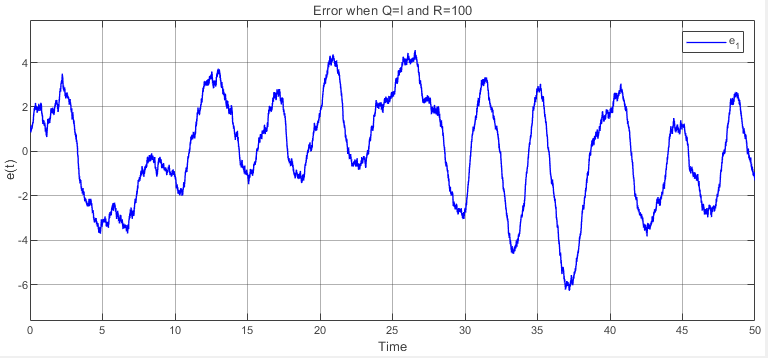
\includegraphics[scale=0.75]{2task_eee1.png}
        \captionsetup{skip=0pt}
        \caption{График $e_1(t)=x_1(t)-\hat{x}_1(t)$ при $L_{I,100}$}
        \label{fig:2task_eee1}
    \end{figure}
    \begin{figure}[H]
        \centering
        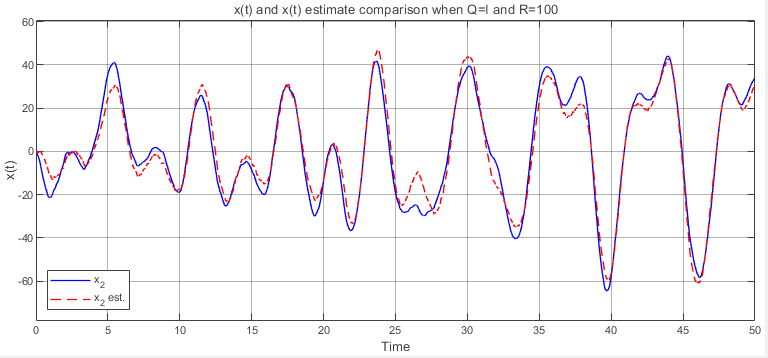
\includegraphics[scale=0.75]{2task_xxx2.png}
        \captionsetup{skip=0pt}
        \caption{График $x_2(t),\hat{x}_2(t)$ при $L_{I,100}$}
        \label{fig:2task_xxx2}
    \end{figure}
    \begin{figure}[H]
        \centering
        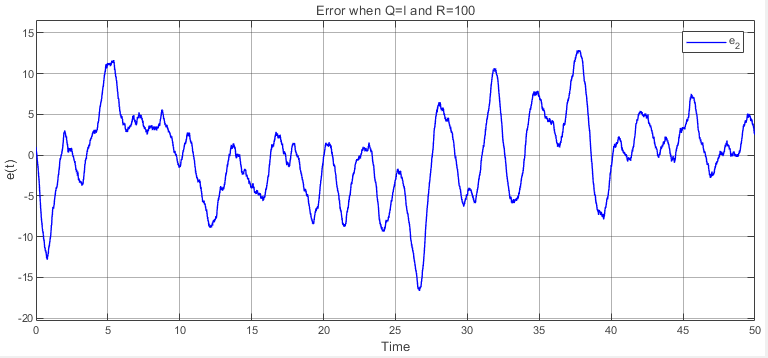
\includegraphics[scale=0.75]{2task_eee2.png}
        \captionsetup{skip=0pt}
        \caption{График $e_2(t)=x_2(t)-\hat{x}_2(t)$ при $L_{I,100}$}
        \label{fig:2task_eee2}
    \end{figure}
    \begin{figure}[H]
        \centering
        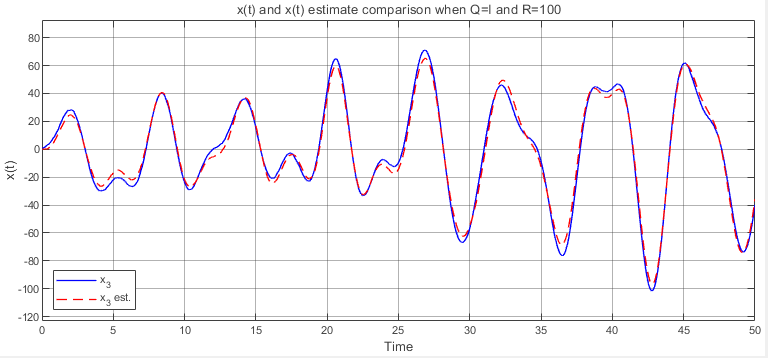
\includegraphics[scale=0.75]{2task_xxx3.png}
        \captionsetup{skip=0pt}
        \caption{График $x_3(t),\hat{x}_3(t)$ при $L_{I,100}$}
        \label{fig:2task_xxx3}
    \end{figure}
    \begin{figure}[H]
        \centering
        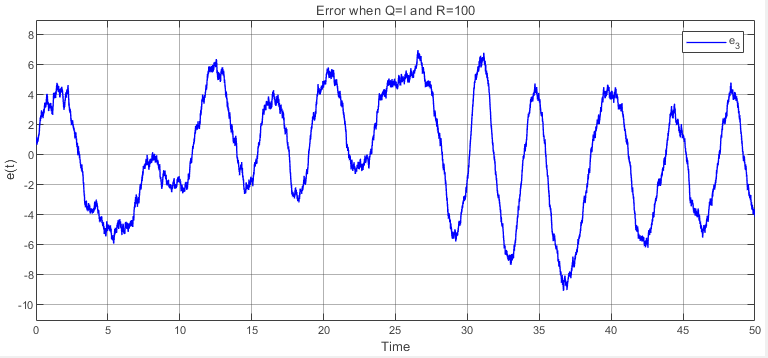
\includegraphics[scale=0.75]{2task_eee3.png}
        \captionsetup{skip=0pt}
        \caption{График $e_3(t)=x_3(t)-\hat{x}_3(t)$ при $L_{I,100}$}
        \label{fig:2task_eee3}
    \end{figure}
    \begin{figure}[H]
        \centering
        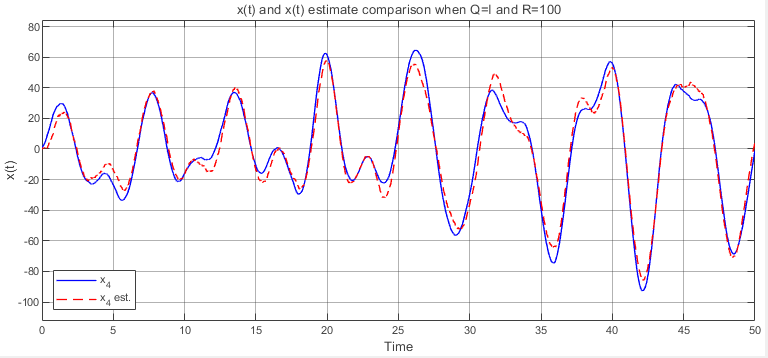
\includegraphics[scale=0.75]{2task_xxx4.png}
        \captionsetup{skip=0pt}
        \caption{График $x_4(t),\hat{x}_4(t)$ при $L_{I,100}$}
        \label{fig:2task_xxx4}
    \end{figure}
    \begin{figure}[H]
        \centering
        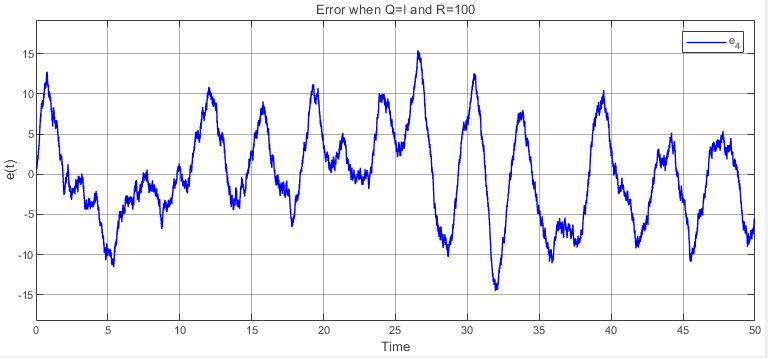
\includegraphics[scale=0.75]{2task_eee4.png}
        \captionsetup{skip=0pt}
        \caption{График $e_4(t)=x_4(t)-\hat{x}_4(t)$ при $L_{I,100}$}
        \label{fig:2task_eee4}
    \end{figure}


    \subsection{Сравнение результатов}
    Возмущение $f(t)$ имеет меньшую амплитуду, чем помеха $\xi(t)$, т.е. $f(t)<\xi(t)$.
    При $Q>R$ наблюдатель верит в то, что в среднем больше случайное возмущение $f$,
    чем случайная помеха $\xi$. При $Q<R$ ситуация обратная
    -- наблюдатель меньше верит датчикам, чем прошлым состояниям объекта.
    На графиках при $Q<R$ видим, что наблюдатель достаточно уверенно ошибается
    в повторении поведения системы, так как не верит показаниям $y$,
    т.е. избыточно фильтрует сигнал; при $Q>R$ наоборот, наблюдатель недостаточно фильтрует
    сигнал, в результате воспроизведение поведения системы шумное, хотя траектория более точная,
    чем при $Q<R$ (например, сравн. рис. \ref{fig:2task_xxx2} с \ref{fig:2task_xx2}).
    Результаты при $Q=R$ выглядят усредненно. Наблюдатель точнее повторяет
    поведение системы в сравнении со случаями при $Q<R$ и при этом имеет
    меньше шумов, чем в результатах при $Q>R$ (например, сравн. рис. \ref{fig:2task_x2} с \ref{fig:2task_xx2}, \ref{fig:2task_xxx2}).


    \section{Задание 3. Синтез LQG}
    Рассмотрим систему
    $$
    \begin{cases}
        \dot{x}=Ax+Bu+f,\\
        y=Cx+Du+\xi,
    \end{cases} x(0)=\begin{bmatrix}
        1\\1\\1\\1
    \end{bmatrix},\ A=\begin{bmatrix}
        2 &0 &-4 &2\\
        0 &2 &-2 &4\\
        -4 &-2 &2 &0\\
        2 &4 &0 &2
    \end{bmatrix},\ B=\begin{bmatrix}
        2 &0\\
        4 &0\\
        6 &0\\
        8 &0
    \end{bmatrix},
    $$
    $$
    C=\begin{bmatrix}
        -2 &2 &2 &2\\
        2 &0 &0 &2
    \end{bmatrix}, D=\begin{bmatrix}
        0 &3\\
        0 &1
    \end{bmatrix},
    $$
    где $f(t),\xi(t)$ -- \textit{детерминированные} сигналы (гармонические возмущения).

    
    \subsection{Стабилизируемость и обнаруживаемость}
    Проверим собственные числа матрицы $A$. Программу \texttt{MATLAB} см. листинг \ref{task3}, приложение В
    $$
    \sigma\left( A \right)=\left\{ -4,0,4,8 \right\}
    $$
    Число $\lambda_1=-4$ асимптотически устойчивое, может быть неуправляемым/ненаблюдаемым.
    $\lambda_2=0$ устойчивое, но не асимптотически. Остальные собственные числа неустойчивые,
    требуется управляемость/наблюдаемость. Найдем $A_J,B_J,C_J$
    $$
    A_J=\begin{bmatrix}
        0     &0     &0     &0\\
     0    &-4     &0     &0\\
     0     &0     &8     &0\\
     0     &0     &0     &4
    \end{bmatrix},\ B_J=\begin{bmatrix}
        3     &0\\
    -1     &0\\
     2     &0\\
     4     &0
    \end{bmatrix},\ C_J=\begin{bmatrix}
        0     &0     &0     &8\\
     4     &0     &4     &0
    \end{bmatrix};
    $$
    Полностью нулевых строк в $B_J$ нет, поэтому система полностью управляема,
    стабилизируема. В $C_J$ нулевому столбцу соответствует число $-4$ в $A_J$ --
    система не полностью наблюдаема, обнаруживаема.


    \subsection{Схема моделирования системы}
    Построим схему моделирования системы, замкнутой регулятором, состоящим из
    наблюдателя состояния $\dot{\hat{x}}=A\hat{x}+\left(B+LD\right)u+L\left(C\hat{x}-y\right)$ и закона управления $u=K\hat{x}$.
    Снимаем осциллограммы $u(t),x(t),\hat{x}(t),e(t)$.
    \begin{figure}[H]
        \centering
        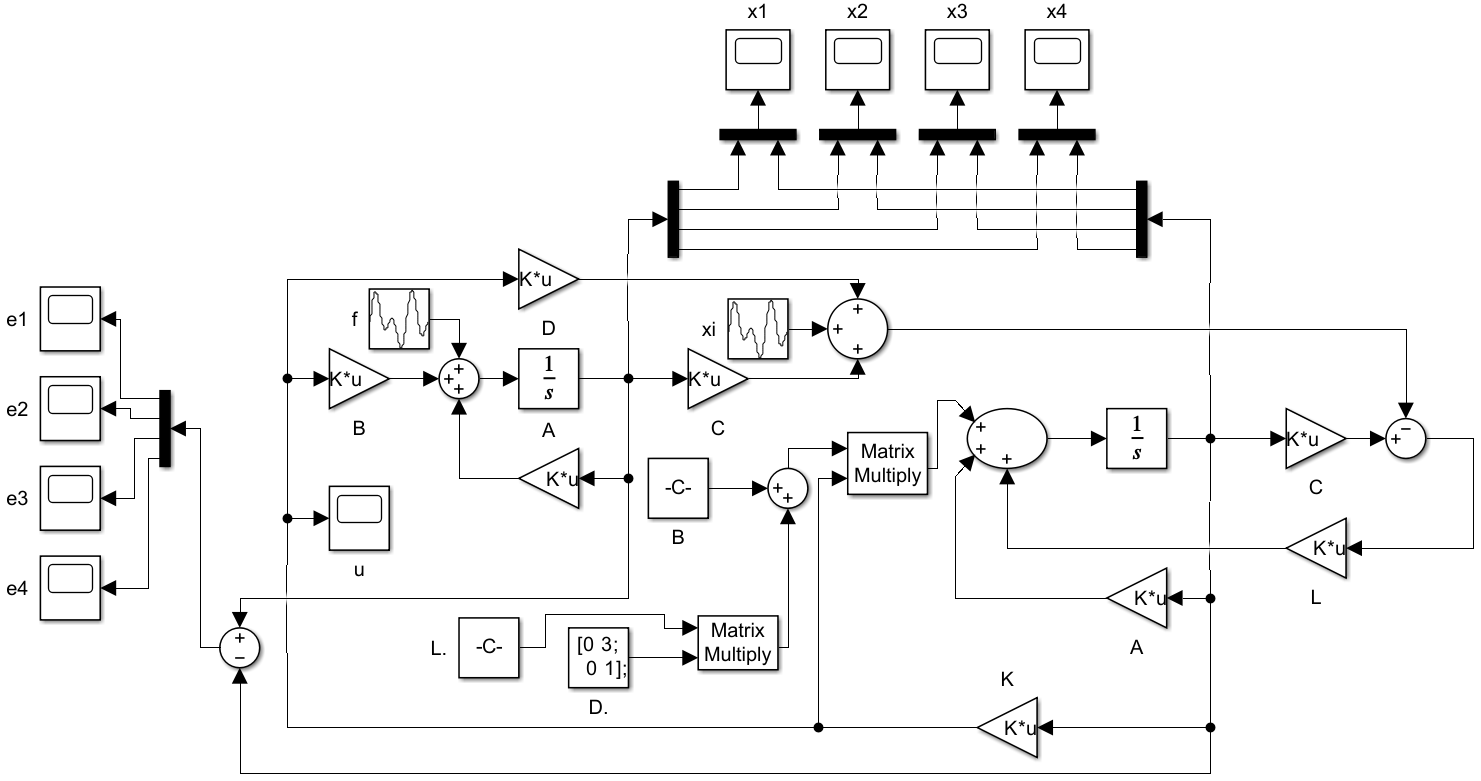
\includegraphics[scale=0.4]{3task_scheme.png}
        \captionsetup{skip=0pt}
        \caption{Схема моделирования системы, замкнутой регулятором, состоящим из наблюдателя состояния и закона управления}
        \label{fig:3task_scheme}
    \end{figure}
    
    
    \subsection{Пары матриц для регулятора и наблюдателя}
    Зададимся парами матриц $\left( Q_K,R_K \right)$ для регулятора и $\left( Q_L,R_L \right)$
    для наблюдателя. Пускай нам важнее затраты на управление, чем время процесса,
    а наблюдатель меньше доверяет датчикам, чем прошлым состояниям объекта. Тогда
    $$
    Q_K=\begin{bmatrix}
        1 &0 &0 &0\\
        0 &1 &0 &0\\
        0 &0 &1 &0\\
        0 &0 &0 &1
    \end{bmatrix},\ R_K=\begin{bmatrix}
        10 &0\\
        0 &10
    \end{bmatrix},\ Q_L=\begin{bmatrix}
        2 &0 &0 &0\\
        0 &2 &0 &0\\
        0 &0 &2 &0\\
        0 &0 &0 &2
    \end{bmatrix},\ R_L=\begin{bmatrix}
        1 &0\\
        0 &1
    \end{bmatrix};
    $$


    \subsection{Синтез регулятора}
    Синтезируем матрицу регулятора с помощью матричного уравнения типа Риккати аналогично предыдущим заданиям
    $$
    K=\begin{bmatrix}
        -10.2086   &-5.2443    &9.8924   &-5.5605\\
         0         &0         &0         &0
    \end{bmatrix},
    $$
    $$
    \sigma\left( A+BK \right)=\left\{ -4,-4.8643,-1.5367,-8.1226 \right\};
    $$
    Регулятор синтезирован корректно.


    \subsection{Синтез наблюдателя}
    Синтезируем матрицу коррекции наблюдателя с помощью матричного уравнения типа Риккати
    аналогично предыдущим заданиям
    $$
    L=\begin{bmatrix}
        1.3660   &-4.7979\\
   -1.3660   &-6.2121\\
   -1.3660    &6.2121\\
   -1.3660   &-4.7979
    \end{bmatrix},
    $$
    $$
    \sigma\left( A+LC \right)=\left\{ -4,-2.6486,-6.9282,-8.5431 \right\};
    $$
    Наблюдатель синтезирован корректно.


    \subsection{Компьютерное моделирование}
    Выполним компьютерное моделирование с нулевыми начальными условиями
    наблюдателя $$\hat{x}(0)=\begin{bmatrix}
        0\\ 0\\ 0\\ 0
    \end{bmatrix}$$ Построим график формируемого регулятором
    управления $u(t)$, сравнительные графики $x(t)$ и $\hat{x}(t)$,
    а также график ошибки наблюдателя $e(t) = x(t) -\hat{x}(t)$.
    Шумы примем такими
    $$
    f(t)=0.1\sin\left( \dfrac{\pi}{3}t \right)-0.3\cos\left( \dfrac{\pi}{3}t \right),
    $$
    $$
    \xi(t)=-0.5\sin\left( \dfrac{\pi}{3}t \right)+0.2\cos\left( \dfrac{\pi}{3}t \right);
    $$
    Результаты представлены на рис. \ref{fig:3task_u}--\ref{fig:3task_e4}
    \begin{figure}[H]
        \centering
        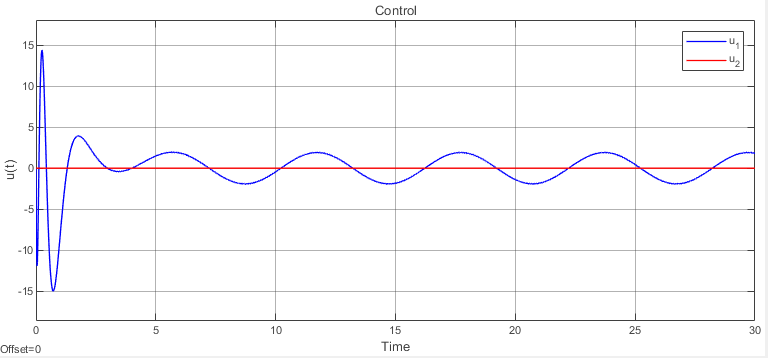
\includegraphics[scale=0.75]{3task_u.png}
        \captionsetup{skip=0pt}
        \caption{График управления $u(t)$}
        \label{fig:3task_u}
    \end{figure}
    \begin{figure}[H]
        \centering
        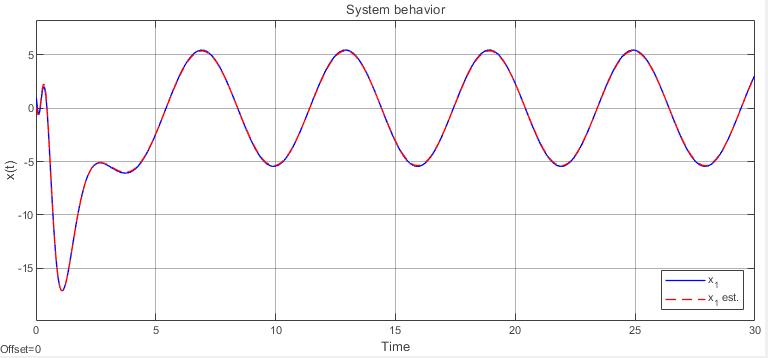
\includegraphics[scale=0.75]{3task_x1.png}
        \captionsetup{skip=0pt}
        \caption{График $x_1(t),\hat{x}_1(t)$}
        \label{fig:3task_x1}
    \end{figure}
    \begin{figure}[H]
        \centering
        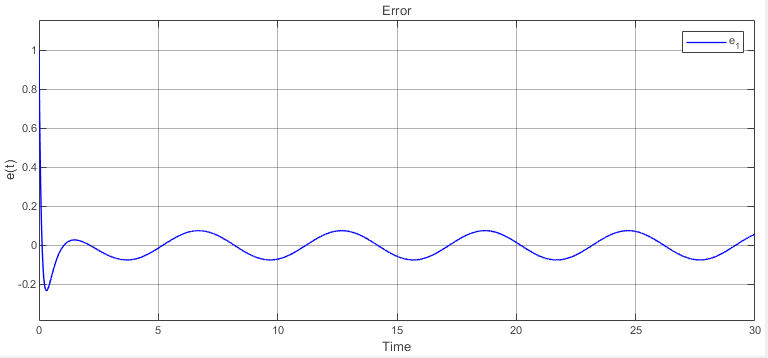
\includegraphics[scale=0.75]{3task_e1.png}
        \captionsetup{skip=0pt}
        \caption{График $e_1(t)=x_1(t)-\hat{x}_1(t)$}
        \label{fig:3task_e1}
    \end{figure}
    \begin{figure}[H]
        \centering
        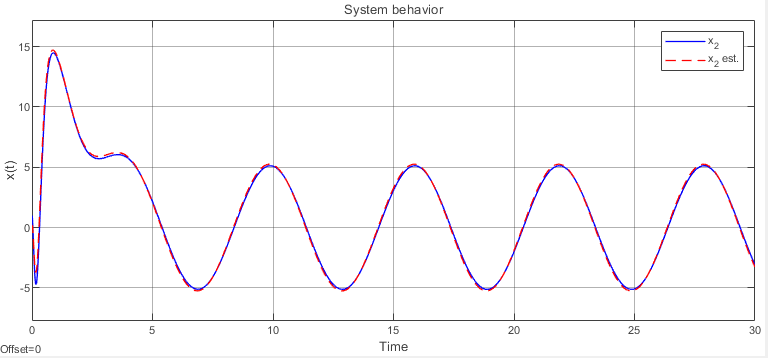
\includegraphics[scale=0.75]{3task_x2.png}
        \captionsetup{skip=0pt}
        \caption{График $x_2(t),\hat{x}_2(t)$}
        \label{fig:3task_x2}
    \end{figure}
    \begin{figure}[H]
        \centering
        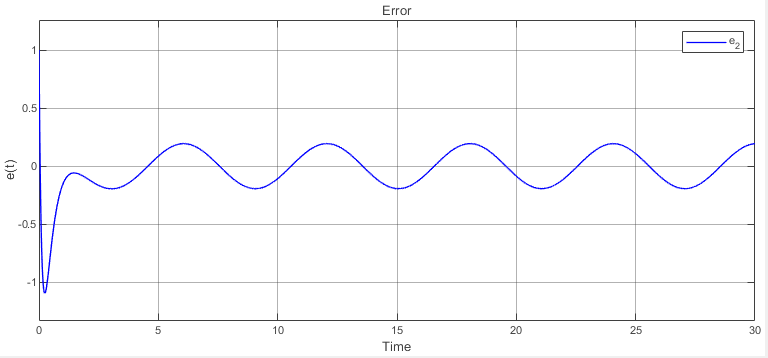
\includegraphics[scale=0.75]{3task_e2.png}
        \captionsetup{skip=0pt}
        \caption{График $e_2(t)=x_2(t)-\hat{x}_2(t)$}
        \label{fig:3task_e2}
    \end{figure}
    \begin{figure}[H]
        \centering
        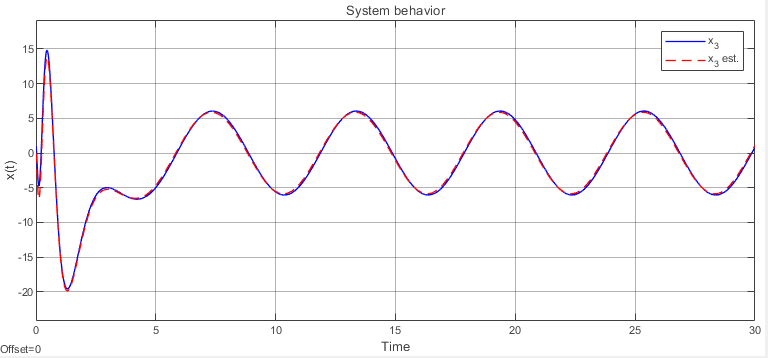
\includegraphics[scale=0.75]{3task_x3.png}
        \captionsetup{skip=0pt}
        \caption{График $x_3(t),\hat{x}_3(t)$}
        \label{fig:3task_x3}
    \end{figure}
    \begin{figure}[H]
        \centering
        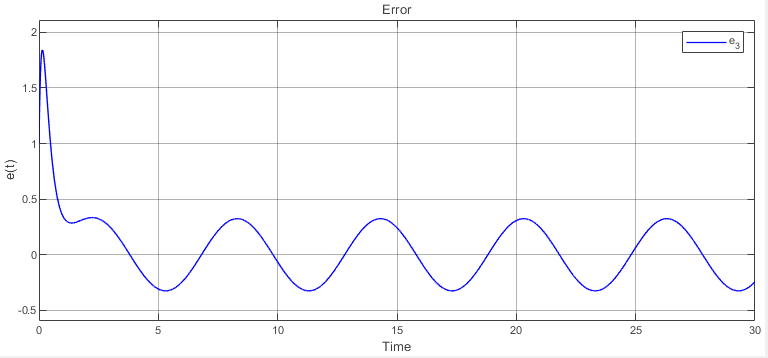
\includegraphics[scale=0.75]{3task_e3.png}
        \captionsetup{skip=0pt}
        \caption{График $e_3(t)=x_3(t)-\hat{x}_3(t)$}
        \label{fig:3task_e3}
    \end{figure}
    \begin{figure}[H]
        \centering
        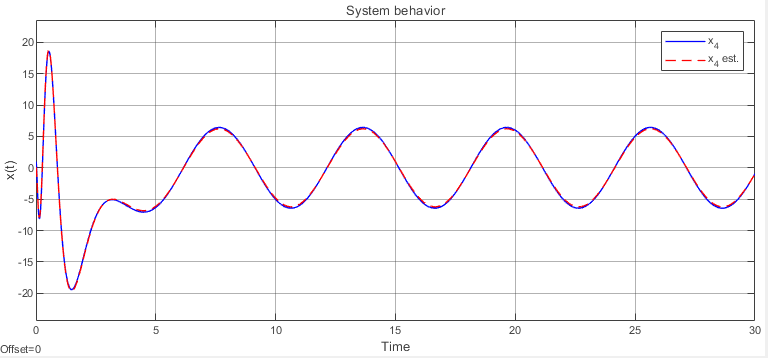
\includegraphics[scale=0.75]{3task_x4.png}
        \captionsetup{skip=0pt}
        \caption{График $x_4(t),\hat{x}_4(t)$}
        \label{fig:3task_x4}
    \end{figure}
    \begin{figure}[H]
        \centering
        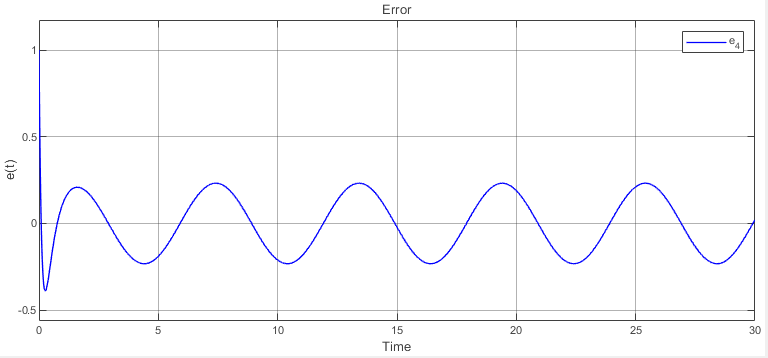
\includegraphics[scale=0.75]{3task_e4.png}
        \captionsetup{skip=0pt}
        \caption{График $e_4(t)=x_4(t)-\hat{x}_4(t)$}
        \label{fig:3task_e4}
    \end{figure}

    
    \subsection{Описание результатов}
    Наблюдатель достаточно хорошо воспроизводит истинное поведение системы, но присутствует устоявшаяся ошибка.
    Регулятор не привел $x(t)$ к нулю, но ему удалось стабилизировать систему
    к незатухающим колебаниям (без роста и убывания амплитуды). По управлению
    видим некоторое перерегулирование в начале.


    \section{Вывод}
    В ходе выполнения работы были рассмотрены виды оптимальных
    регуляторов и наблюдателей -- LQR, фильтр Калмана, LQG.
    Для LQR и фильтра Калмана были исследованы различные пары
    значений матриц, использующихся для решения матричного уравнения типа Риккати.
    В каждом задании было проведено моделирование системы,
    результаты были сравнены. Полученные графики подтверждают корректность расчетов и рассуждений.


    \section{Приложение А}
    \begin{lstlisting}[label=task1, caption={Программа для задания 1}]
    % plant parameters
    A = [5 2 7; 2 1 2; -2 -3 -4];
    B = [3; 1; -1];
    x0 = [1;1;1];

    % A matrix eigenvalues
    eig_A = eig(A)

    % Jordan matrix
    [P_J, A_J] = jordan(A);
    P_Jre(:,1) = P_J(:,1);
    P_Jre(:,2) = imag(P_J(:,2));
    P_Jre(:,3) = real(P_J(:,3));
    A_Jre = P_Jre^-1 * A * P_Jre
    B_jre = P_Jre^-1 * B

    % solving Riccati
    a = 4;
    Q= a*eye(3);
    R = a*1;

    [P,K,e]=icare(A,B,Q,R);
    P
    K=-inv(R)*B'*P
    e=eig(A+B*K)

    % quality functional
    J_min = x0'*P*x0
    \end{lstlisting}


    \section{Приложение Б}
    \begin{lstlisting}[label=task2, caption={Программа для задания 2}]
    % plant parameters
    A = [0 1 0 1;
        -26 -7 20 -11;
         0 1 -1 2;
         16 4 -14 8];
    C = [-1 0 1 -1];

    % A matrix eigenvalues
    eig_A = eig(A)

    % Jordan matrix
    [P_J, A_J] = jordan(A);
    P_Jre(:,1) = real(P_J(:,1));
    P_Jre(:,2) = imag(P_J(:,2));
    P_Jre(:,3) = real(P_J(:,3));
    P_Jre(:,4) = imag(P_J(:,4));
    A_Jre = P_Jre^-1 * A * P_Jre
    C_jre = C*P_Jre

    % solving Riccati
    a = 100;
    Q= a*eye(4);
    R = a*1;

    [P,L,e]=icare(A',C',Q,R);
    P
    L=-P*C'*R^-1
    e=eig(A+L*C)
    \end{lstlisting}


    \section{Приложение В}
    \begin{lstlisting}[label=task3, caption={Программа для задания 3}]
    % plant parameters
    A = [2 0 -4 2;
         0 2 -2 4;
        -4 -2 2 0;
         2 4 0 2];
    B= [2 0;
        4 0;
        6 0;
        8 0];
    C= [-2 2 2 2;
        2 0 0 2];
    D=[0 3;
    0 1];

    % A matrix eigenvalues
    eig_A = eig(A)

    % Jordan matrix
    [P_J, A_J] = jordan(A)
    B_J = P_J^-1 * B
    C_J = C*P_J

    % regulator
    Qr= eye(4);
    Rr = 10*eye(2);

    [Pr,K,e]=icare(A,B,Qr,Rr);
    K=-inv(Rr)*B'*Pr
    ek=eig(A+B*K)

    % observer
    Ql= 2*eye(4);
    Rl = eye(2);

    [Pl,L,e]=icare(A',C',Ql,Rl);
    L=-Pl*C'*Rl^-1
    el=eig(A+L*C)
    \end{lstlisting}
\end{document}